
\question{Déterminer la vitesse \emph{V}, supposée constante, à
laquelle doit se déplacer le robot en ligne droite pour réaliser la
tâche au maximum en \emph{T\textsubscript{m }}secondes en fonction de
\emph{L}, \(\mathcal{l}\), \emph{T\textsubscript{m }}et
\emph{T\textsubscript{p}}. Faire l'application numérique pour une durée
\emph{T\textsubscript{m }}de 320 secondes.}

\begin{texteCache}

 Pour déplacer les 4 rangées, il faut 4 déplacements de la zone 1 vers
  la zone 2 (distance \emph{L} = 10m) et 3 déplacements de la zone 2
  vers la zone 1 (distance \emph{L+}$l$ = 10,5m)

  La durée \emph{T\textsubscript{m}} correspond donc à
  \(T_{m} = 8T_{p} + \frac{7L + 3 l}{V}\) soit
  \(V = \frac{7L + 3 l}{T_{m} - 8T_{p}}\) AN~:
  \(V = 0,89\ m.s^{- 1}\)


\end{texteCache}


\question{À l'aide des informations ci-dessus, compléter les chaînes
d'énergie et d'information pour le déplacement du robot.}

\ifthenelse{\boolean{corrige}}{
\begin{center}
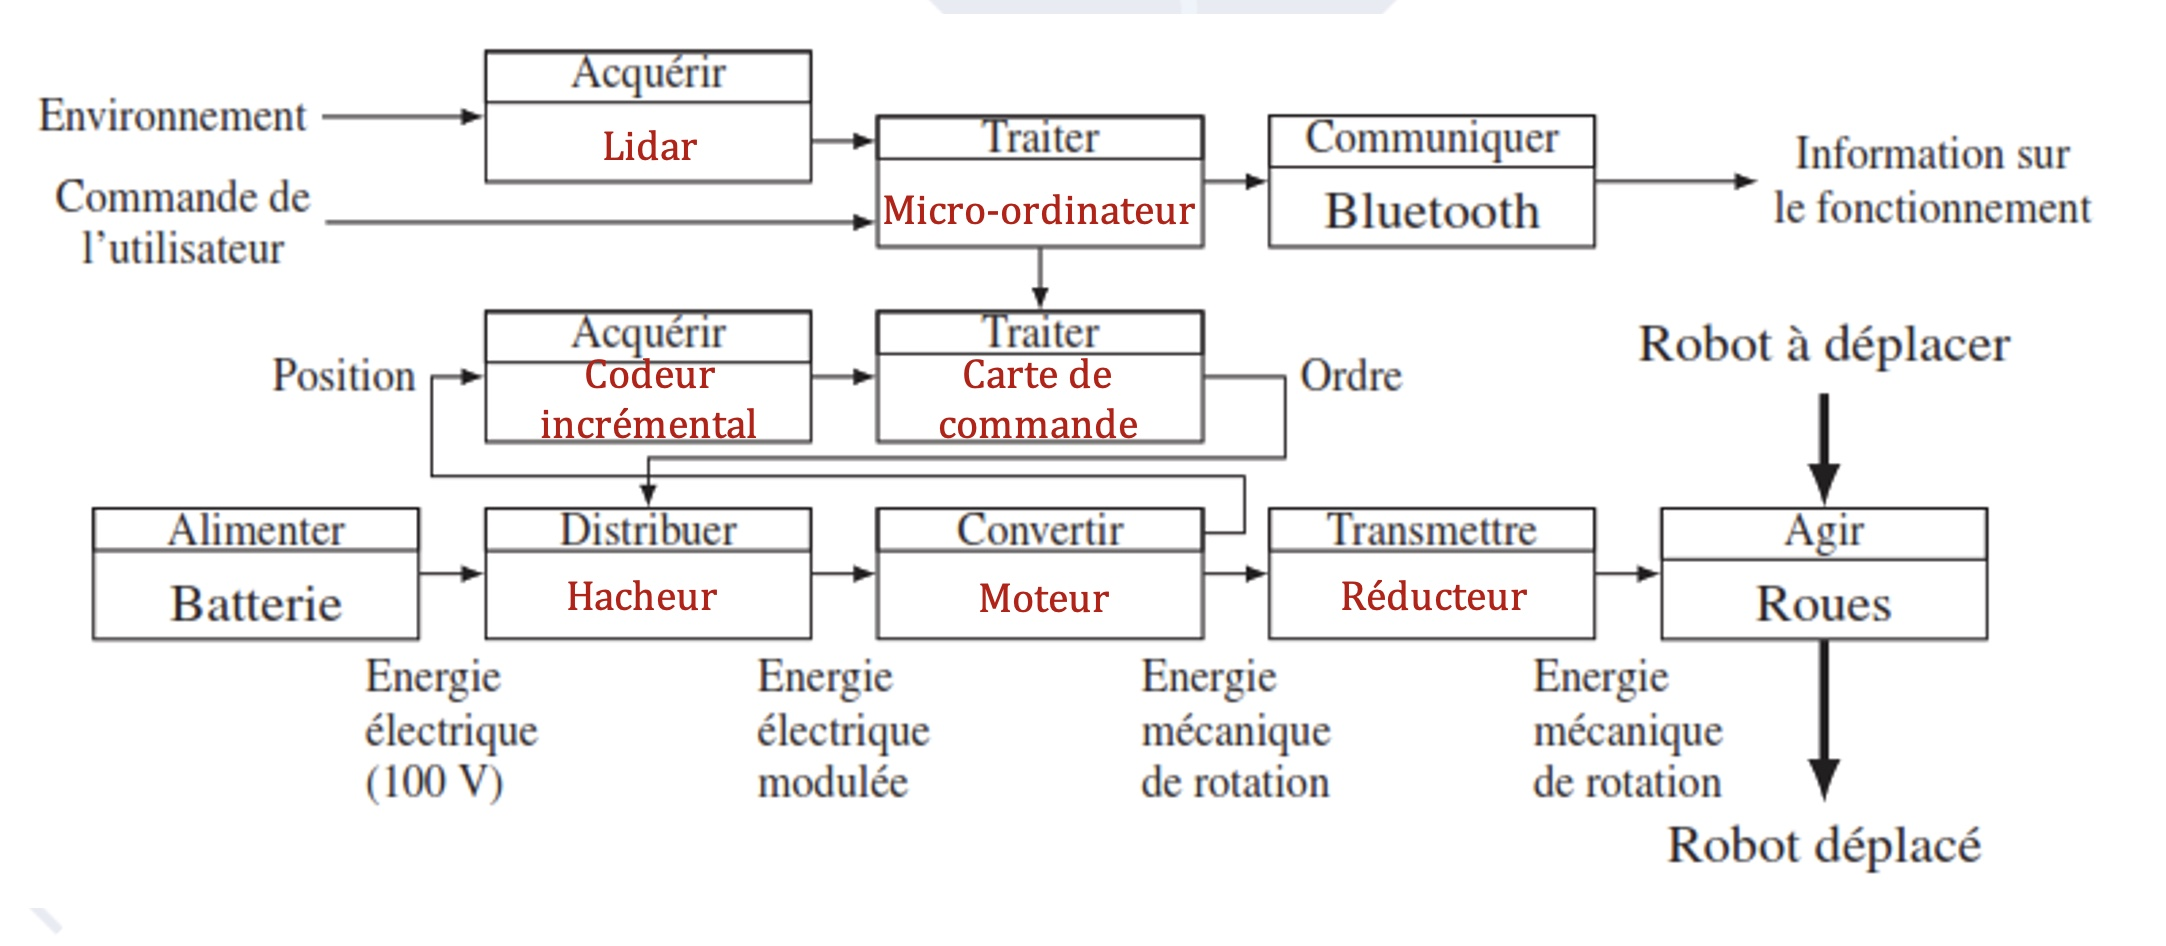
\includegraphics[width=0.95\textwidth]{images/CF1.jpg}
\end{center}
}
{
\begin{center}
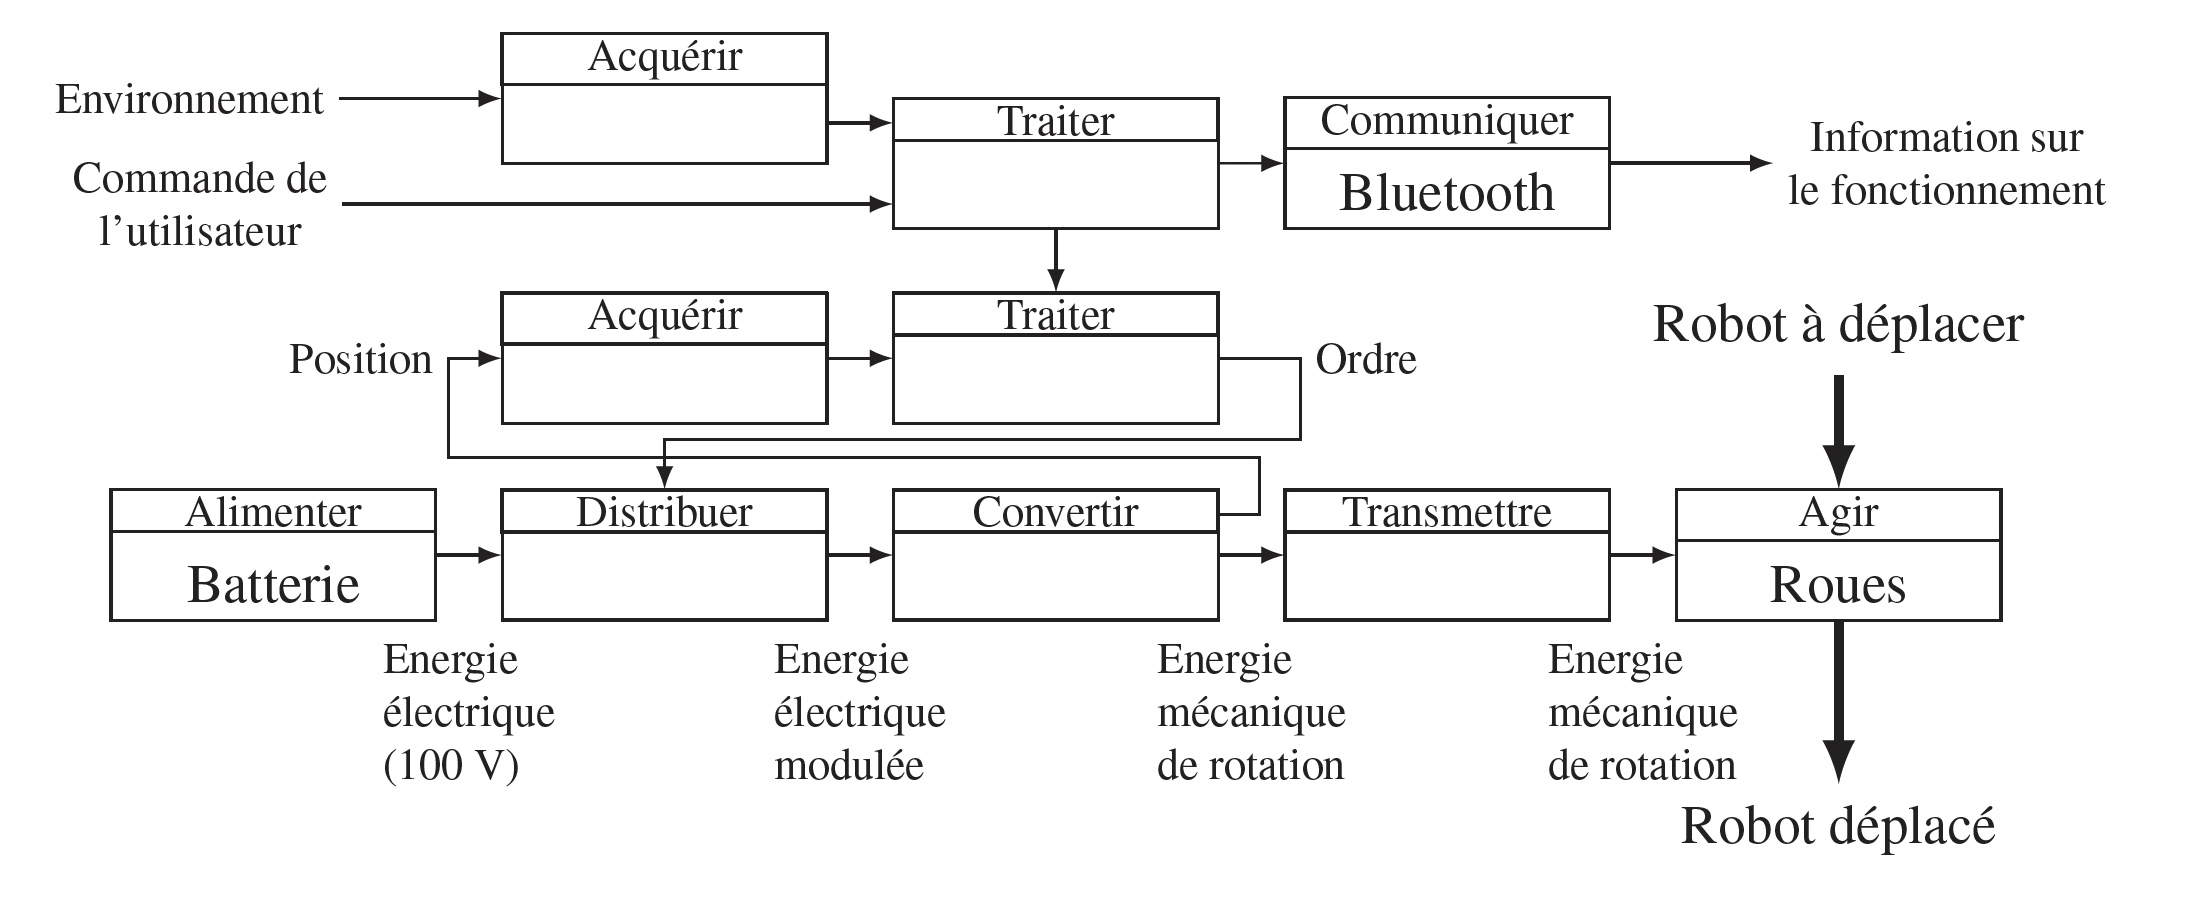
\includegraphics[width=0.95\textwidth]{images/CF0.jpg}
\end{center}
}


\question{A l'aide du diagramme des exigences de la figure \ref{fig4}, donner l'identifiant de l'exigence permettant de vérifier le critère de vitesse maximale}

\begin{texteCache}
Il s'agit de l'exigence 1.1
\end{texteCache}

\question{Vérifier que les éléments choisis permettent de respecter
le critère de vitesse maximale défini dans le diagramme des exigences.}

\begin{texteCache}

On veut vérifier que la vitesse maximale de 1,1
  m.s\textsuperscript{-1} puisse être atteinte~:

  \(V_{\max} = \omega_{m}.k_{r}.r = 3000.\frac{2\pi}{60}.\frac{1}{40}.0,15 = 1,18\ m.s^{- 1}\)
  L'exigence 1.5.2 est donc vérifiée avec ce moteur

\vspace{2cm}
\end{texteCache}


\question{Déterminer l'expression du temps $\delta t$ pour respecter
le déplacement souhaité en fonction de $D$, $T$ et
$\V_{max}$. Faire l'application numérique.}



\begin{texteCache}

La distance parcourue D correspond à l'aire sous la courbe, soit~:

  \(D = \frac{V_{\max}.\delta t}{2} + V_{\max}.\left( T - 2\delta t \right) + \frac{V_{\max}.\delta t}{2} = V_{\max}.\left( T - \delta t \right)\)

  D'où \(\delta t = - \frac{D}{V_{\max}} + T\) AN~: \(\delta t = 0,91s\)

\vspace{5cm}
\end{texteCache}

\question{Déterminer l'équation différentielle vérifiée par
\(v\left( t \right)\) avec \(u_{m}\left( t \right)\) comme entrée. On montrera qu'elle pourra se mettre sous la forme : $A\dfrac{d v(t)}{dt}+B\cdot v(t)=u_m(t)$ et on identifiera A et B en fonction des constantes du problèmes.}

\begin{texteCache}



  

  Avec \(C_{r}\left( t \right) = 0\), les équations (2) et (3) donnent~:
  \(i_{m}\left( t \right) = \frac{C_{m}\left( t \right)}{k_{m}} = \frac{1}{2k_{m}}.J.\frac{d\omega_{m}\left( t \right)}{\text{dt}}\)

  L'équation (4) devient, après dérivation par rapport au temps~:
  \(\frac{\text{dv}\left( t \right)}{\text{dt}} = k_{t}.\frac{d\omega_{m}(t)}{\text{dt}}\)

  L'équation (1) s'écrit alors~:
  \(u_{m}\left( t \right) = R_{m}.\frac{1}{2k_{m}}.J.\frac{1}{k_{t}}.\frac{\text{dv}\left( t \right)}{\text{dt}} + \frac{k_{m}}{k_{t}}.v\left( t \right)\)

  Soit
  \(\text{\ \ }\frac{R_{m}.J}{2k_{m}k_{t}}.\frac{\text{dv}\left( t \right)}{\text{dt}} + \frac{k_{m}}{k_{t}}.v\left( t \right) = u_{m}\left( t \right)\text{\ \ }\)
  (*)
  
  \vspace{3cm}
  \end{texteCache}
  
  
  \question{Vérifier que \(v\left( t \right) = \alpha_{0}(t - \tau_{m} + \tau_{m}e^{- t/\tau_{m}})\)
est solution de l'équation différentielle pour une consigne de tension
\(u_{m}\left( t \right) = \frac{u_{0}}{\delta t}t\) pour $t \geq 0$.}


\begin{texteCache}

  Pour la vérification de la solution, on pose
  
  \begin{itemize}
  \item  \(\frac{R_{m}.J}{2k_{m}k_{t}} = a\)~;
  
  \item  \(\frac{k_{m}}{k_{t}} = b\)~;


 \item  \(\frac{u_{0}}{\delta t} = c\)~:
  \end{itemize}
 

  L'équation (*) devient
  \(a.\frac{\text{dv}\left( t \right)}{\text{dt}} + b.v\left( t \right) = c\cdot t\)

  On donne
  \(v\left( t \right) = \alpha_{0}(t - \tau_{m} + \tau_{m}e^{- t/\tau_{m}})\)
  donc
  
  \begin{align*}
   \frac{dv(t)}{\text{dt}} = \alpha_{0}(1 - e^{- t/\tau_{m}})
  \end{align*}

  Soit en injectant dans la relation précédente~:
  \(a.\alpha_{0}(1 - e^{- t/\tau_{m}}) + b.\alpha_{0}(t - \tau_{m} + \tau_{m}e^{- t/\tau_{m}}) = c\cdot t\)
\vspace{3cm}
  \end{texteCache}
  
  \question{On donnera l'expression de \(\alpha_{0}\) et \(\tau_{m}\) en fonction de
\(u_{0}\), \(\delta t\) et des constantes intervenant dans les
équations du moteur.}


\begin{texteCache}

  Par identification, on trouve alors~:
  
  
  \(\alpha_{0} = \frac{c}{b} = \frac{u_{0}.k_{t}}{\delta tk_{m}}\)
  
  
  et \(\tau_{m} = \frac{a}{b} = \frac{R_{m}.J}{2k_{m}^2}\)
  
  \vspace{3cm}


\end{texteCache}


\question{Compléter la partie permettant de définir les fonctions \texttt{F(y,t}) et \texttt{u\_m(t)} qui permettent d'obtenir le la liste \texttt{vt} par la méthode d'Euler.}

\ifthenelse{\boolean{corrige}}{
\begin{center}
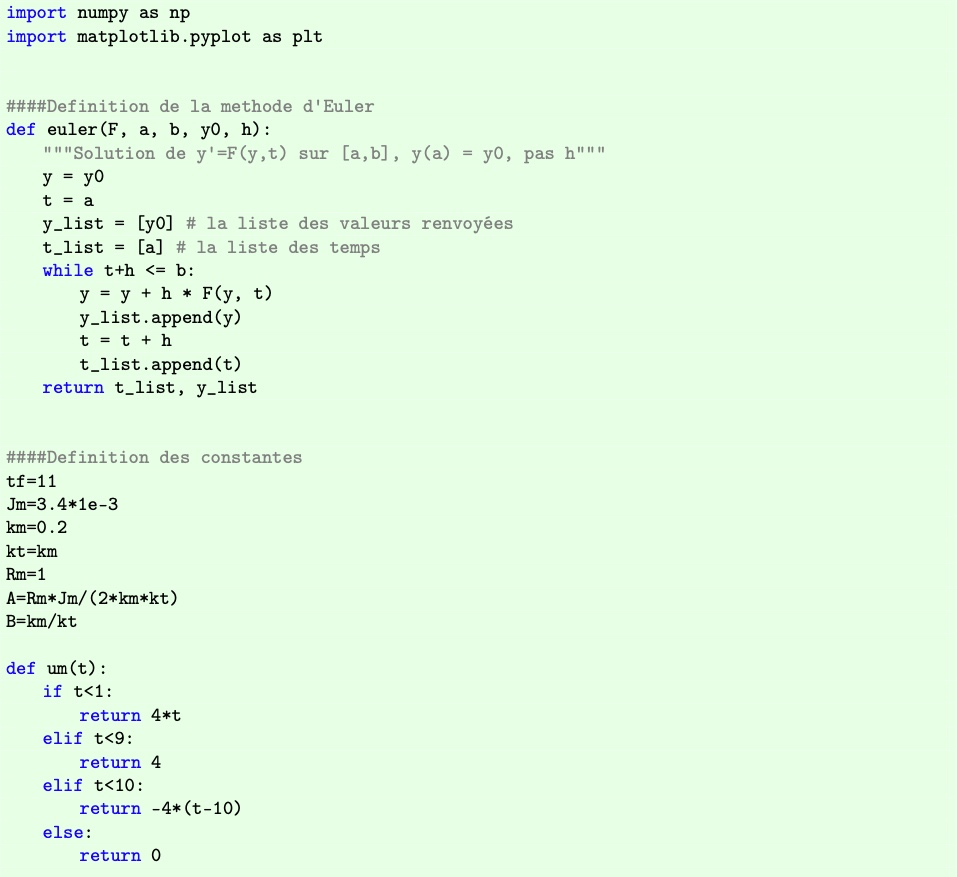
\includegraphics[width=0.9\textwidth]{images/prog_corrige1}\\
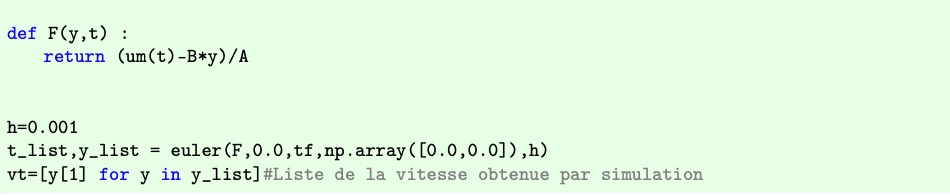
\includegraphics[width=0.9\textwidth]{images/prog_corrige2}
\end{center}
}
{
\begin{center}
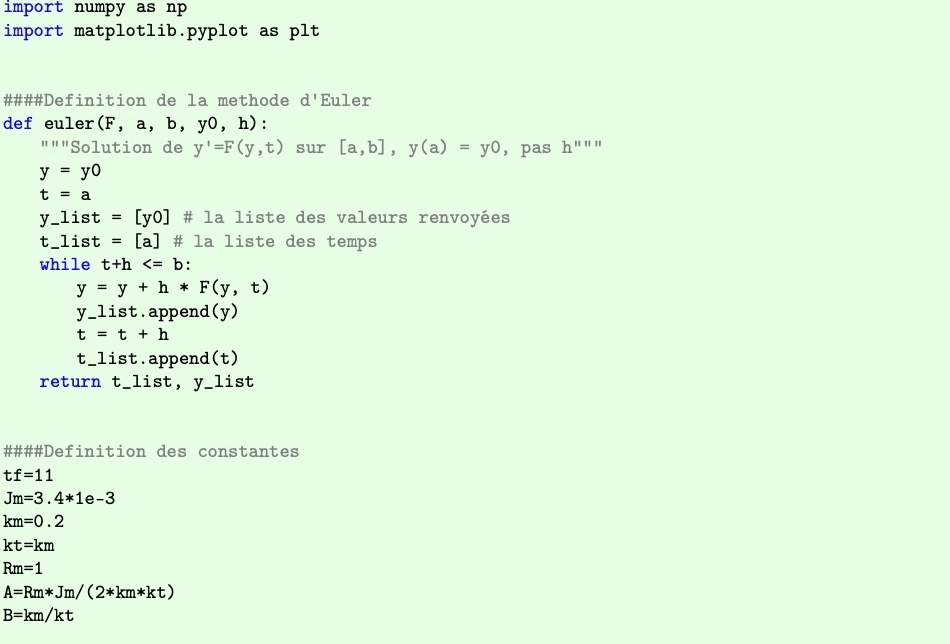
\includegraphics[width=0.9\textwidth]{images/prog_non_corrige1}\\
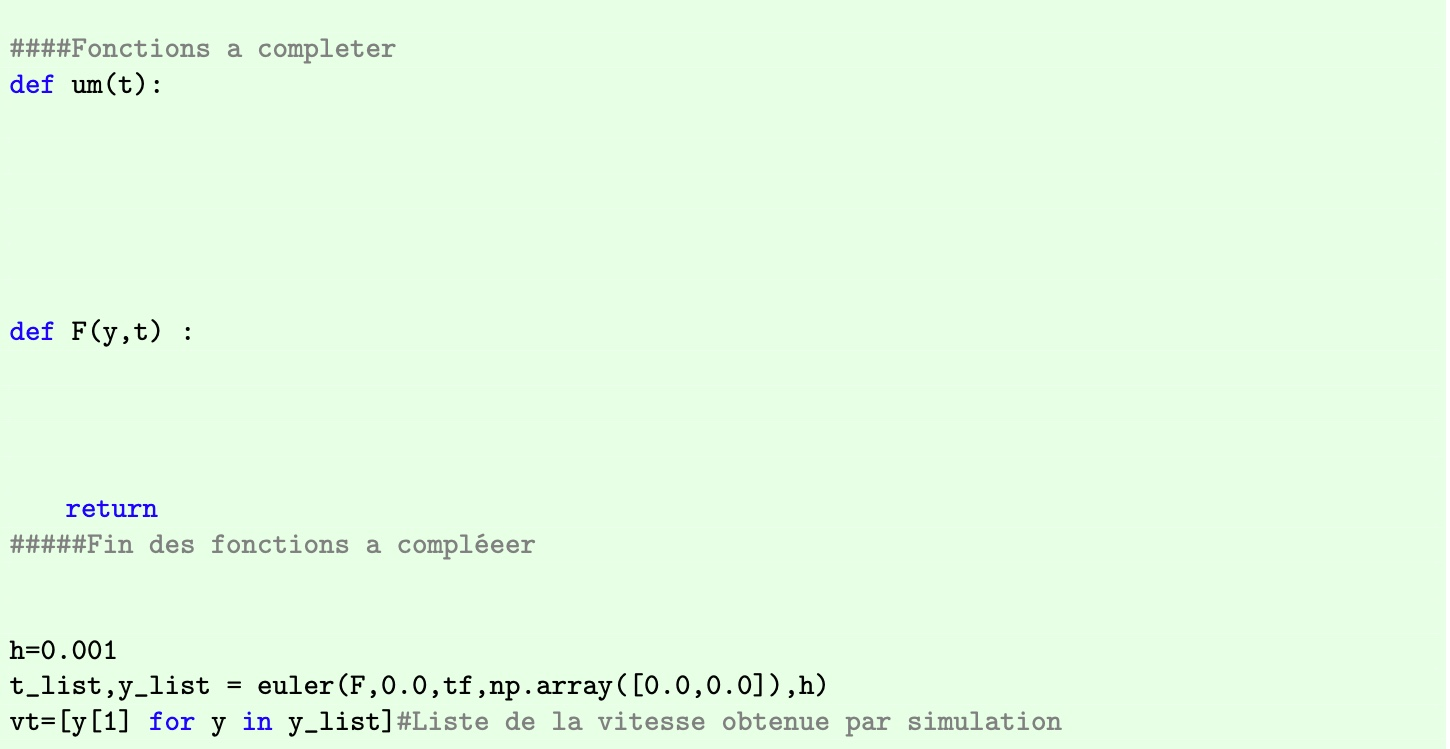
\includegraphics[width=0.9\textwidth]{images/prog_non_corrige2}
\end{center}
}


\question{Proposer une méthode d'intégration numérique permettant d'obtenir cette courbe à partie de la liste \texttt{vt}. Écrire sous la forme d'une fonction codée en python3 les instructions correspondantes.}

\begin{texteCache}
On peut utiliser la méthode des trapézes : 

\begin{center}
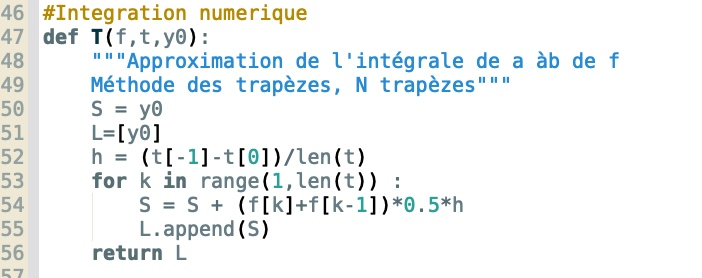
\includegraphics[width=0.9\textwidth]{images/trapeze_num}
\end{center}

\end{texteCache}
%\ifthenelse{\boolean{corrige}}{
%\begin{lstlisting}
%import numpy as np
%import matplotlib.pyplot as plt
%
%
%####Definition de la methode d'Euler
%def euler(F, a, b, y0, h):
%    """Solution de y'=F(y,t) sur [a,b], y(a) = y0, pas h"""
%    y = y0
%    t = a
%    y_list = [y0] # la liste des valeurs renvoyées
%    t_list = [a] # la liste des temps
%    while t+h <= b:
%        y = y + h * F(y, t)
%        y_list.append(y)
%        t = t + h
%        t_list.append(t)
%    return t_list, y_list
%
%
%####Definition des constantes
%tf=11
%Jm=3.4*1e-3
%km=0.2
%kt=km
%Rm=1
%A=Rm*Jm/(2*km*kt)
%B=km/kt
%
%def um(t):
%    if t<1:
%        return 4*t
%    elif t<9:
%        return 4
%    elif t<10:
%        return -4*(t-10)
%    else:
%        return 0
%
%def F(y,t) :
%    return (um(t)-B*y)/A
%    
%    
%h=0.001
%t_list,y_list = euler(F,0.0,tf,np.array([0.0,0.0]),h)
%vt=[y[1] for y in y_list]#Liste de la vitesse obtenue par simulation
%\end{lstlisting}
%}
%{
%sjkhskd
%}
%}
%{
%\newpage
%\begin{lstlisting}
%import numpy as np
%import matplotlib.pyplot as plt
%
%
%####Definition de la methode d'Euler
%def euler(F, a, b, y0, h):
%    """Solution de y'=F(y,t) sur [a,b], y(a) = y0, pas h"""
%    y = y0
%    t = a
%    y_list = [y0] # la liste des valeurs renvoyées
%    t_list = [a] # la liste des temps
%    while t+h <= b:
%        y = y + h * F(y, t)
%        y_list.append(y)
%        t = t + h
%        t_list.append(t)
%    return t_list, y_list
%
%
%####Definition des constantes
%tf=11
%Jm=3.4*1e-3
%km=0.2
%kt=km
%Rm=1
%A=Rm*Jm/(2*km*kt)
%B=km/kt
%
%
%
%####Fonctions a completer
%def um(t):
%
%
%
%
%
%
%def F(y,t) :
%
%
%
%
%    return 
%#####Fin des fonctions a compléeer
%    
%    
%h=0.001
%t_list,y_list = euler(F,0.0,tf,np.array([0.0,0.0]),h)
%vt=[y[1] for y in y_list]#Liste de la vitesse obtenue par simulation
%\end{lstlisting}


\question{En s'aidant de l'expression de la vitesse donnée
précédemment, estimer la valeur de \(\tau_{m}\) à partir de la courbe de
vitesse réelle. Faire apparaître le tracé sur la figure du
\textbf{Document Réponse}.}

\ifthenelse{\boolean{corrige}}{
\begin{center}
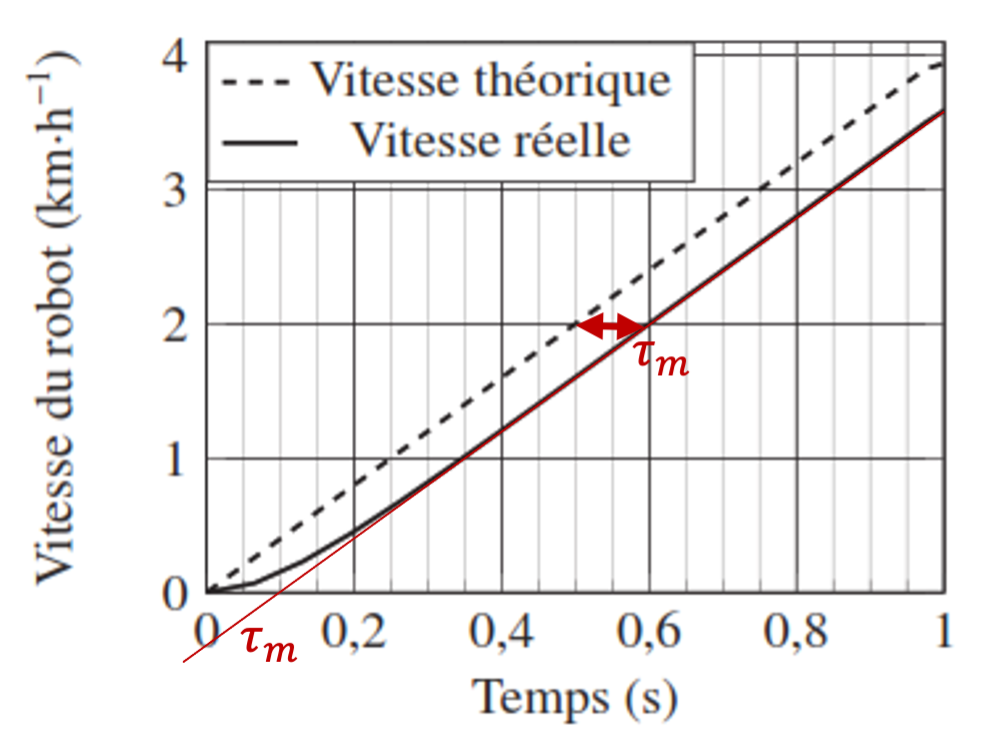
\includegraphics[width=0.6\textwidth]{images/reponse_ramp_corrige.png}
\end{center}
}
{
\begin{center}
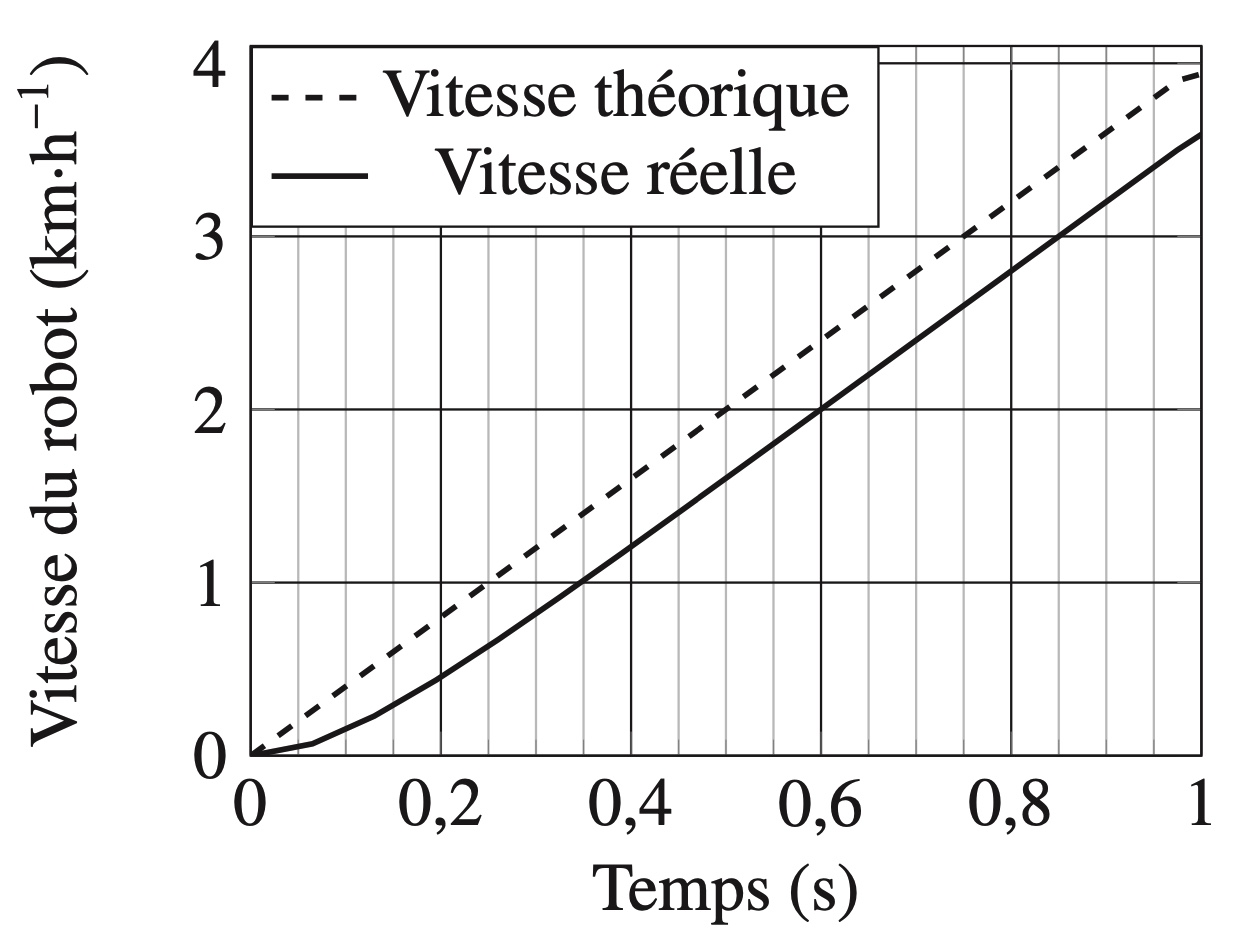
\includegraphics[width=0.6\textwidth]{images/reponse_ramp_0}
\end{center}
}

\begin{texteCache}

On lit sur le graphique $\tau_m=0,1s$.

\vspace{4cm}

\end{texteCache}

\question{À partir des équations (1), (2) et (3), déterminer
la relation \(\Omega_{m}\left( p \right) = H_{m}\left( p \right).U_{m}\left( p \right) + H_{r}\left( p \right).C_{r}\left( p \right)\)
où l'on précisera l'expression de \(H_{m}\left( p \right)\) et
\(H_{r}\left( p \right)\) sous forme canonique.}




\begin{texteCache}
 On écrit les relations dans le domaine de Laplace, avec conditions
  initiales nulles~:

  \(U_{m}\left( p \right) = R_{m}.I_{m}\left( p \right) + k_{m}.\Omega_{m}\left( p \right)\)

  \({2C}_{m}\left( p \right) - C_{r}\left( p \right) = J.p.\Omega_{m}\left( p \right)\)

  \(C_{m}\left( p \right) = k_{m}.I_{m}\left( p \right)\)

  En combinant les relations sans faire intervenir \emph{Im(p),} on
  obtient facilement~:


\[\Omega_{m}\left( p \right) = \frac{2k_{m}}{R_{m}.Jp + 2k_{m}^2}U_{m}\left( p \right) - \frac{R_{m}}{R_{m}.Jp + 2k_{m}^2}C_{r}\left( p \right)\]

Sous forme canonique, on a alors~:


\(\ H_{m}\left( p \right) = \frac{\frac{1}{k_{m}}}{\frac{R_{m}.J}{2k_{m}^2}p + 1}\)


et


\(H_{r}\left( p \right) = - \frac{\frac{R_{m}}{2k_{m}^2}}{\frac{R_{m}.J}{2k_{m}^2}\ p + 1}\)

\end{texteCache}

\question{Compléter le schéma-bloc de l'asservissement de vitesse
linéaire du robot en utilisant les indications précédentes.}
%%%%
\ifthenelse{\boolean{corrige}}{
\begin{center}
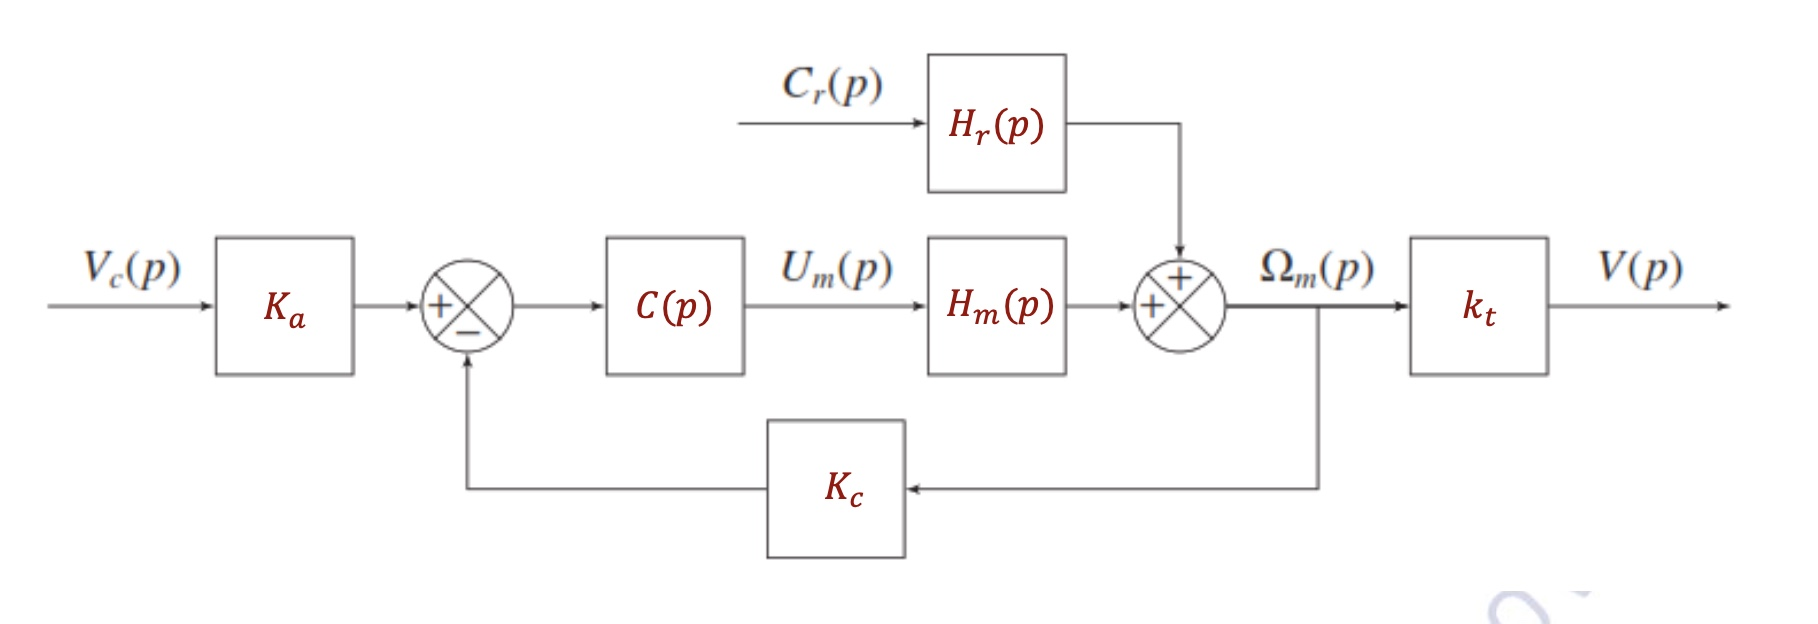
\includegraphics[width=0.9\textwidth]{images/schema_bloc}
\end{center}
}
{
\begin{center}
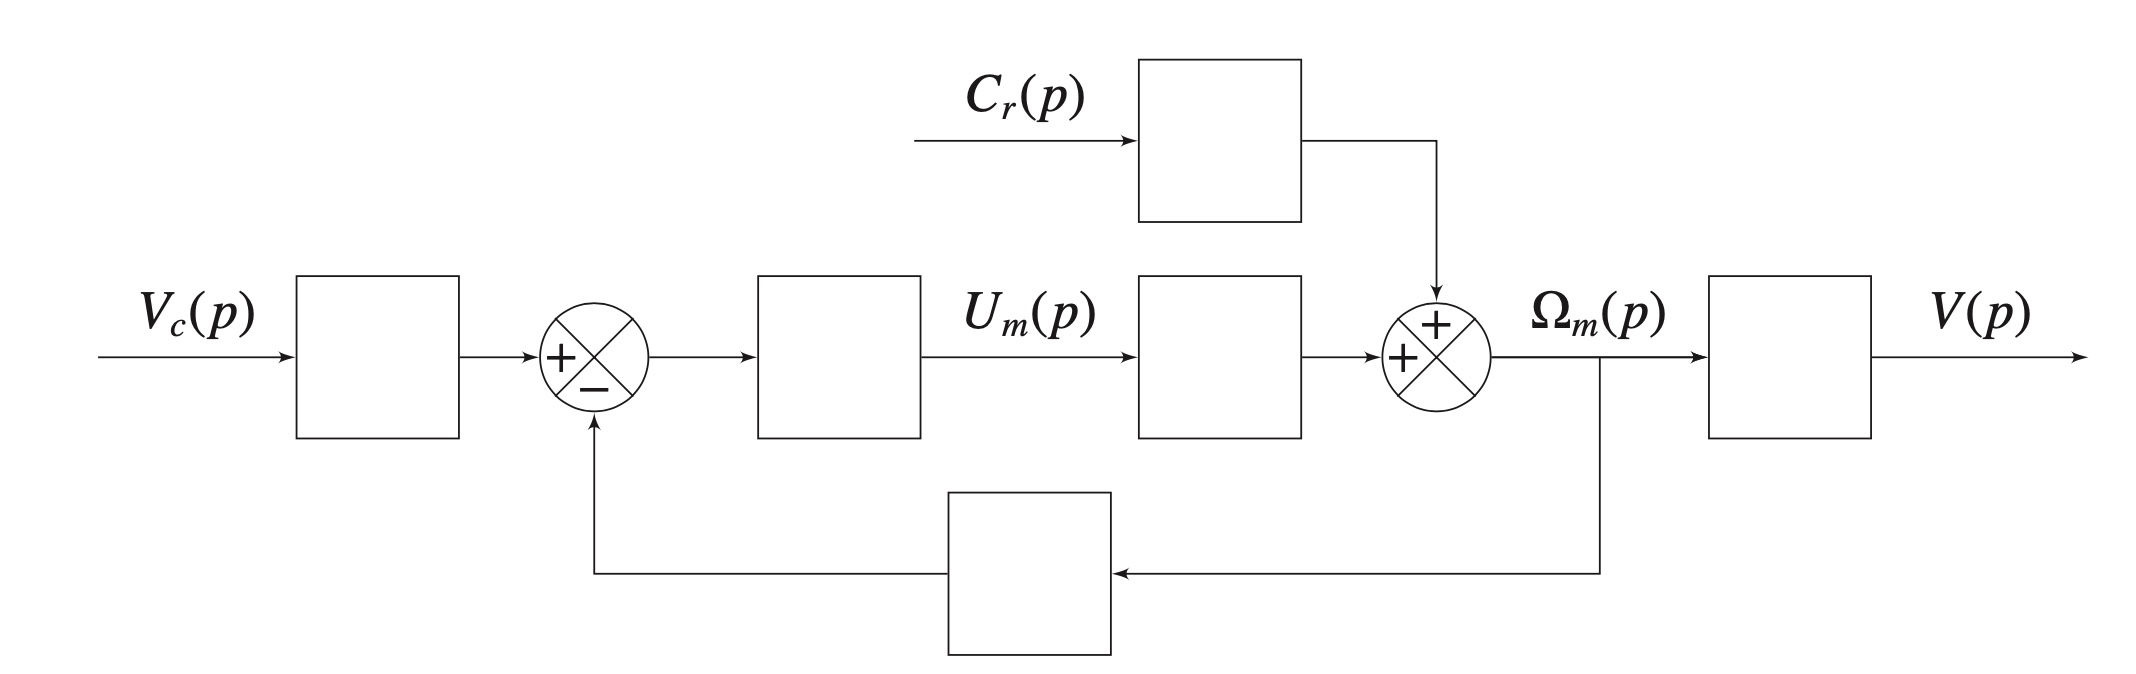
\includegraphics[width=0.9\textwidth]{images/schema_bloc0}
\end{center}
}

\question{Préciser la
valeur numérique de $K_c$ en \emph{inc}/\emph{rad}.
Donner l'expression de $K_a$ permettant d'assurer un
asservissement correct.}

\begin{texteCache}

  \(K_{c} = 628\ \text{inc}/\text{tr} = \frac{628}{2\pi}\text{inc}/\text{rad}\)
  
soit

\begin{align*}
K_{c} \approx 100 inc/rad
\end{align*}


  Pour un asservissement correct, il faut que l'écart en sortie du
  comparateur soit nul lorsque v(t) = v\textsubscript{c}(t), ce qui
  impose \(K_{a} = \frac{K_{c}}{k_{t}}\)


\end{texteCache}

\question{Tracer sur le document réponse le diagramme de Bode asymptotique du correcteur $C(p)$ avec $K_p=1$. Veillez à bien justifier votre réponse.}


\begin{texteCache}
\renewcommand{\arraystretch}{3}

On trouve 2 pulsation caractéristiques identiques. Dans l'ordre croissant $\dfrac{1}{\tau_i}=\dfrac{K_p}{\tau_i=}10 rad/s$.




\begin{center}
\begin{tabular}{|p{1.cm}|p{1.cm}|p{1.cm}|c|p{1.cm}|p{1.cm}|}
\hline 
$\omega$& \multicolumn{2}{c|}{$0 \to \dfrac{1}{\tau_i}$}   & $\dfrac{1}{\tau_i}$ &  \multicolumn{2}{c|}{$\dfrac{1}{\tau_i}\to \infty$}\\ 
\hline 
Tracé asymptotique &  Gain ($dB/dec$) & $\varphi (^\circ)$ & Gain ($dB$) & Gain ($dB/dec$) & $\varphi (^\circ)$  \\ 
\hline 
$\frac{K_{p}}{\tau_i \cdot p}$ & $-20$ & $-90$ & $0$ & $-20$ & $-90$  \\ 
\hline 
$1+\tau_i\cdot p$ & $0$ & $0$ & $0$ & $+20$ & $+90$  \\ 
\hline 
\hline
$H_{BO}(p)$ & $-20$ & $-90$ & $0$ & $0$ & $0$   \\ 
\hline 
\end{tabular} 
\end{center}
\end{texteCache}



\ifthenelse{\boolean{corrige}}{
\begin{center}
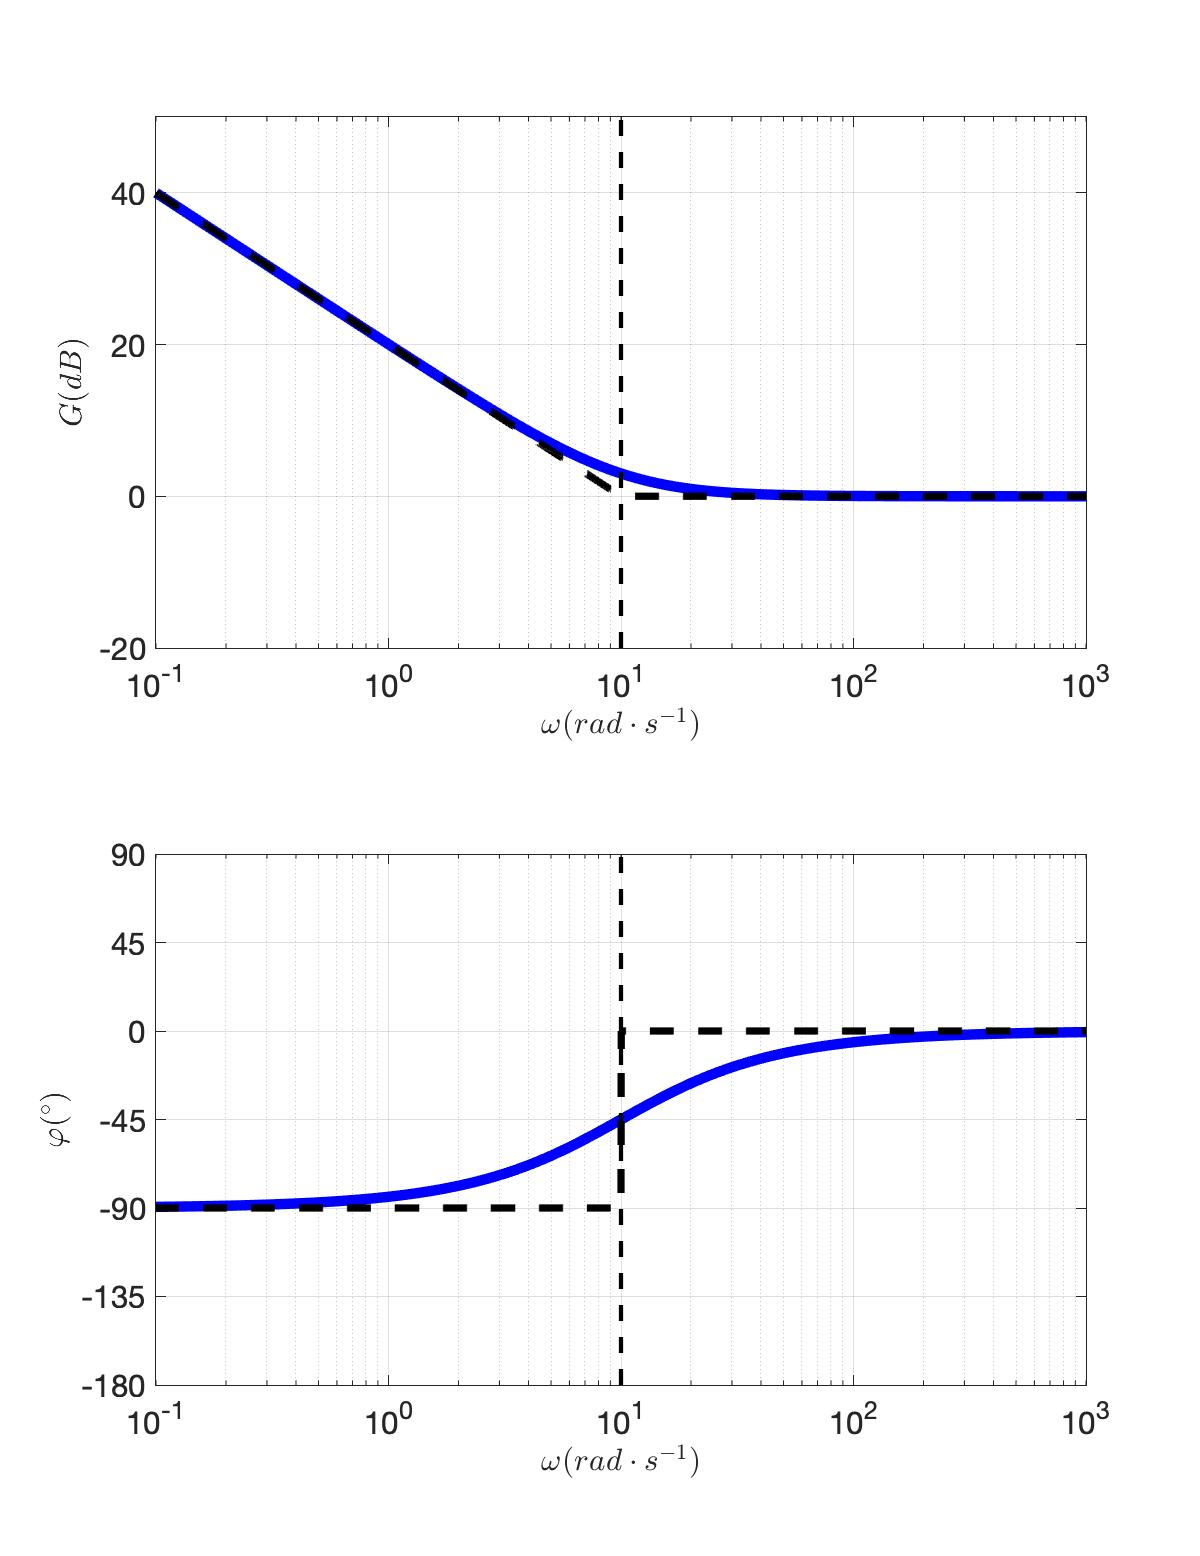
\includegraphics[width=0.9\textwidth]{images/bode_total_PI_2}
\end{center}
}
{
\begin{center}
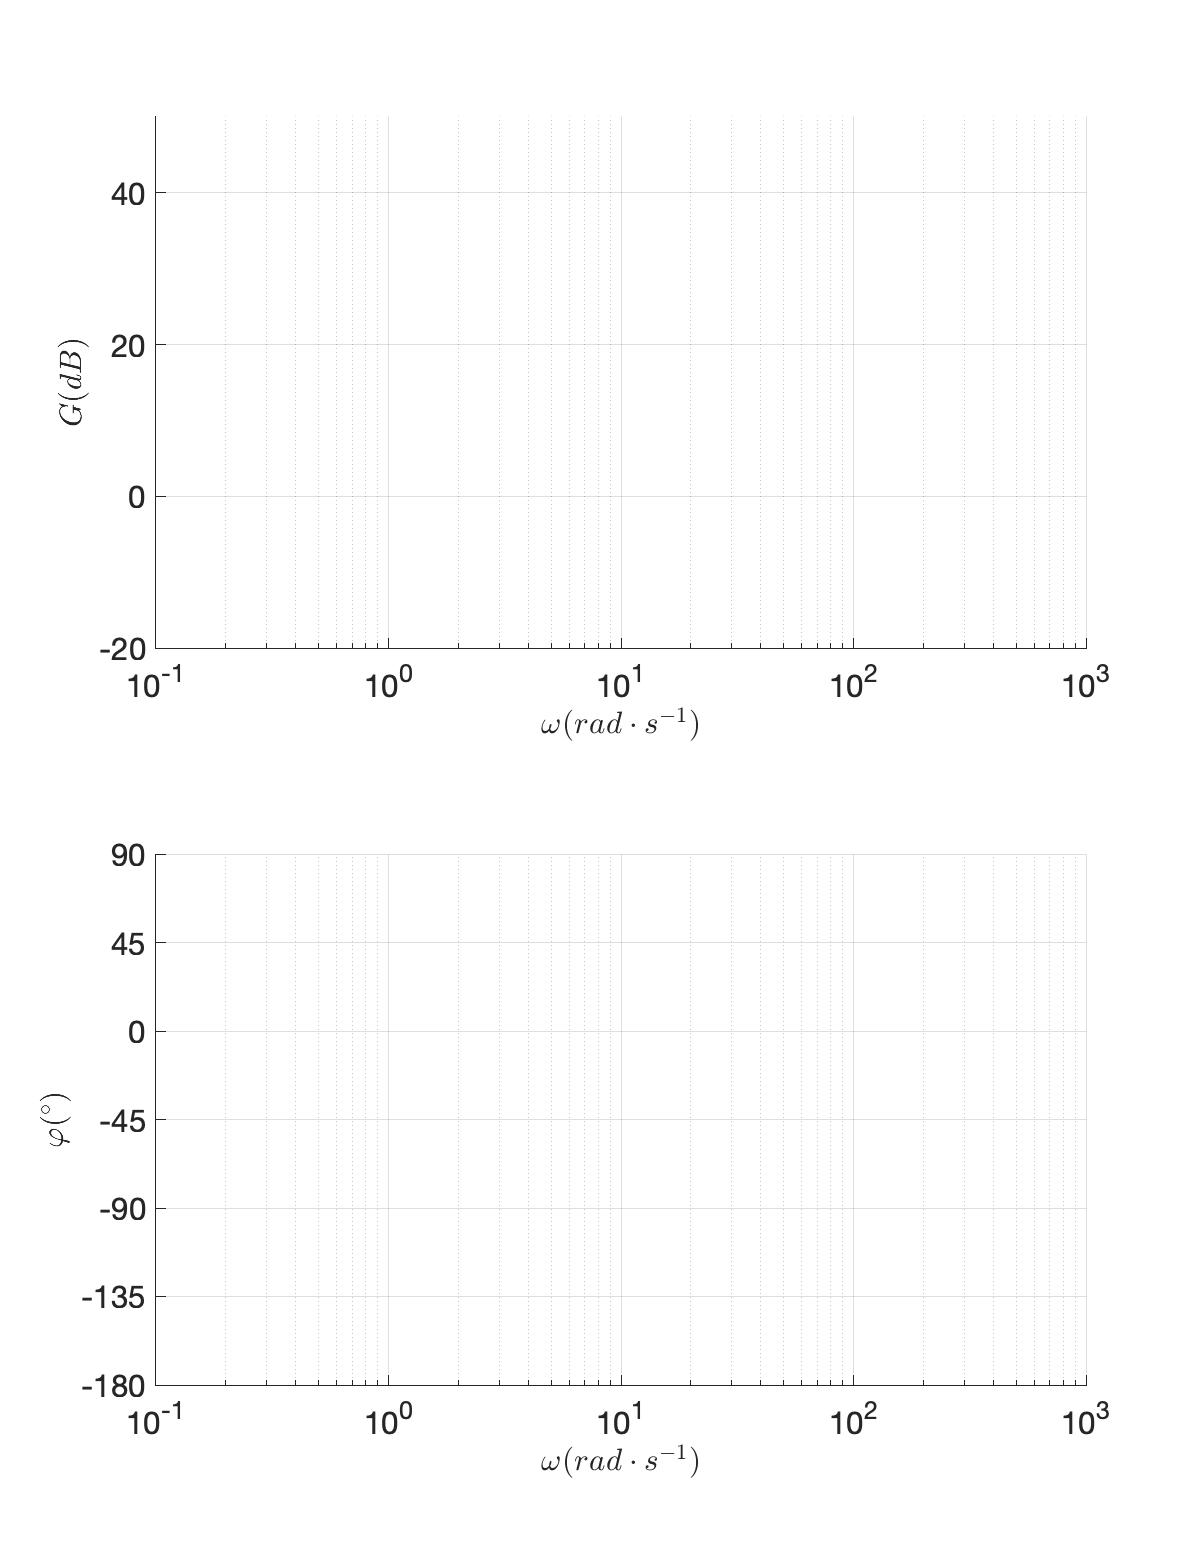
\includegraphics[width=0.9\textwidth]{images/bode_total_PI_0}
\end{center}
}

\question{Calculer la fonction de transfert en boucle fermée du système et la mettre sous forme canonique.}

\begin{texteCache}

\[\frac{V(p)}{V_{c}(p)} = \frac{K_{p}\frac{1 + \tau_{m}p}{\tau_{m}p}.\frac{K_{m}K_{c}}{{1 + \tau}_{m}p}}{1 + K_{p}\frac{1 + \tau_{m}p}{\tau_{m}p}.\frac{K_{m}K_{c}}{{1 + \tau}_{m}p}} = \frac{1}{1 + \frac{\tau_{m}}{K_{p}K_{m}K_{c}}p}\]
\vspace{3cm}
\end{texteCache}

\question{Déterminer la valeur de $K_p$ pour que
le temps de réponse à $5 \%$ en boucle fermée soit égal à $0,3s$.}

\begin{texteCache}
On souhaite \(\text{tr}_{5\%} = 0,3\ s\) , soit
\(\frac{3.\tau_{m}}{K_{p}K_{m}K_{c}} = 0,3\)

On en déduit \(K_{p} = \frac{10.\tau_{m}}{K_{m}K_{c}} = 0,002\)

\vspace{3cm}
\end{texteCache}

\question{Tracer le diagramme de Bode de $FTBO(p)$ avec la valeur de $K_p$ trouvée précédemment. Conclure sur la stabilité du système et donnant les marges de stabilité.}

\begin{texteCache}
Lorsqu'on calcule la FTBO après simplification, on obtient,

\begin{align*}
FTBO(p)=\dfrac{K_pK_mK_c}{\tau_i p}
\end{align*}

Il s'agit donc d'un intégrateur de gain $K_pK_mK_c=500\times 0,002=10 $

Ainsi la pulsation de gain nulle est égale à 10 rad/s et le diagramme en gain possède une pente de $-20db/decade$.

La phase est constante égale à $-90^{\circ}$.

\begin{itemize}
\item \textbf{Marge de phase} : $90^{\circ}$
\item \textbf{Marge de gain} : infinie
\end{itemize}

\end{texteCache}


\ifthenelse{\boolean{corrige}}{
\begin{center}
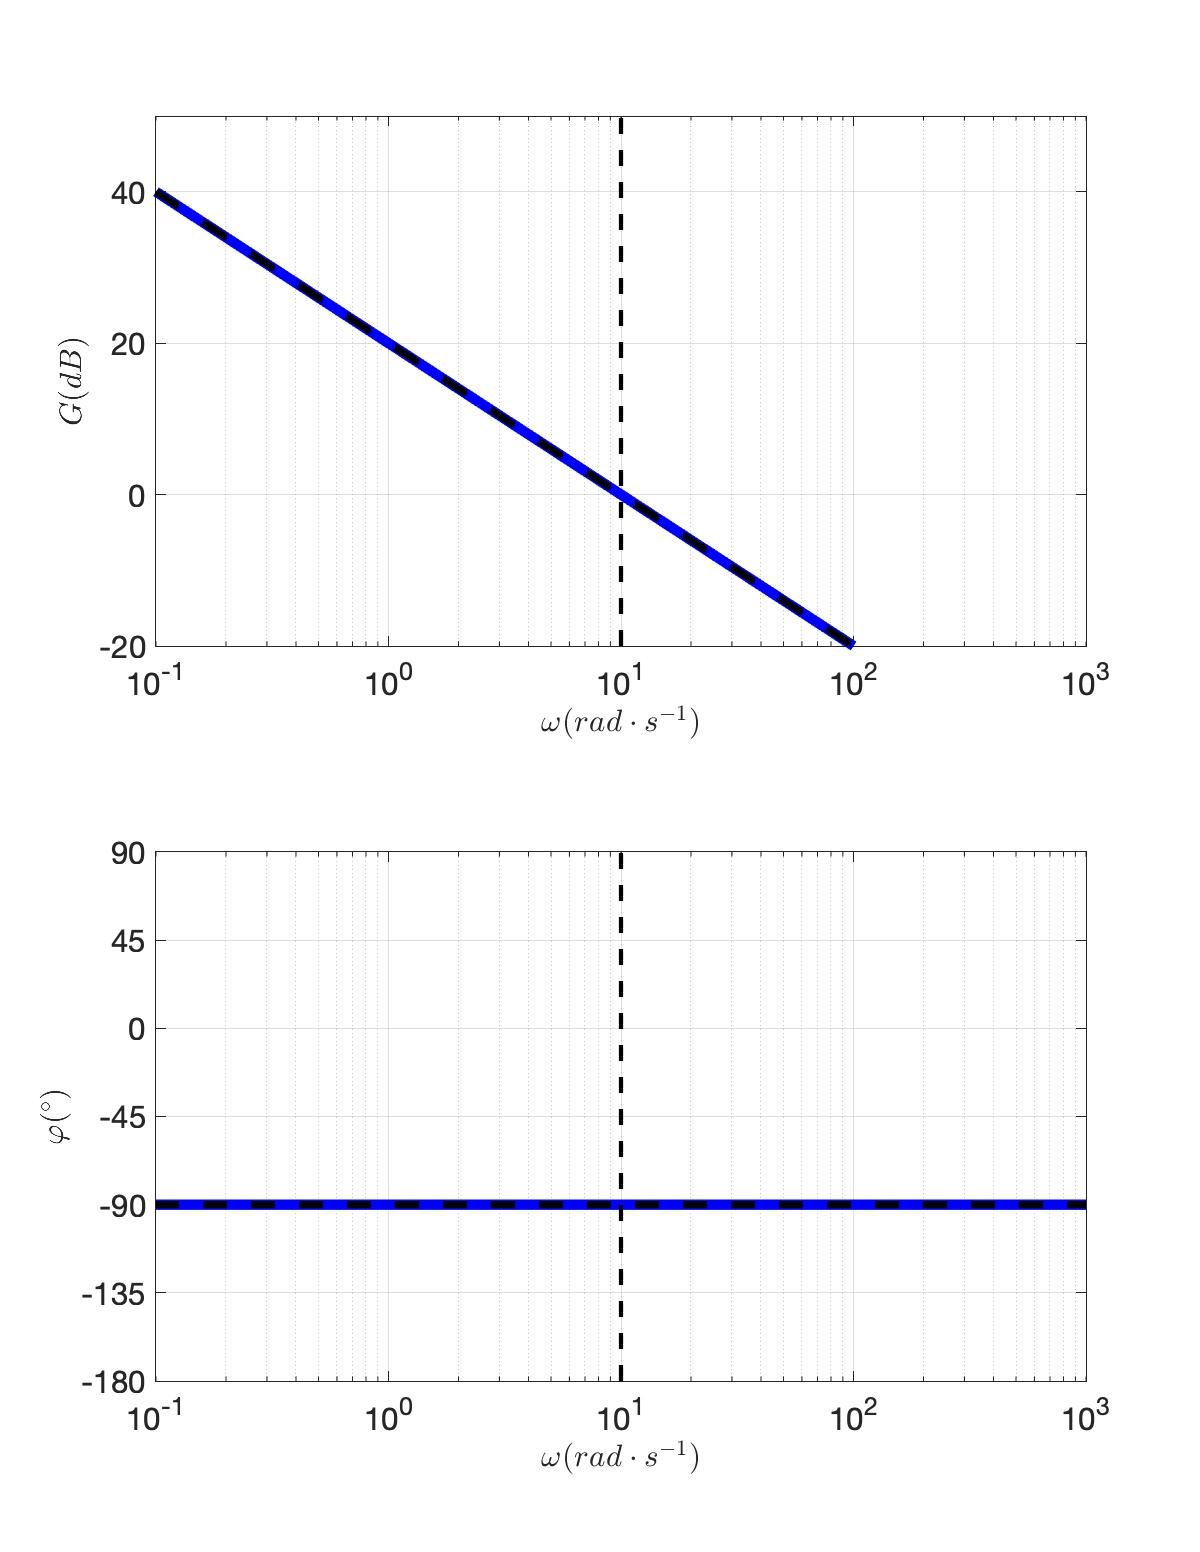
\includegraphics[width=0.9\textwidth]{images/bode_total_BO_2}
\end{center}
}
{
\begin{center}
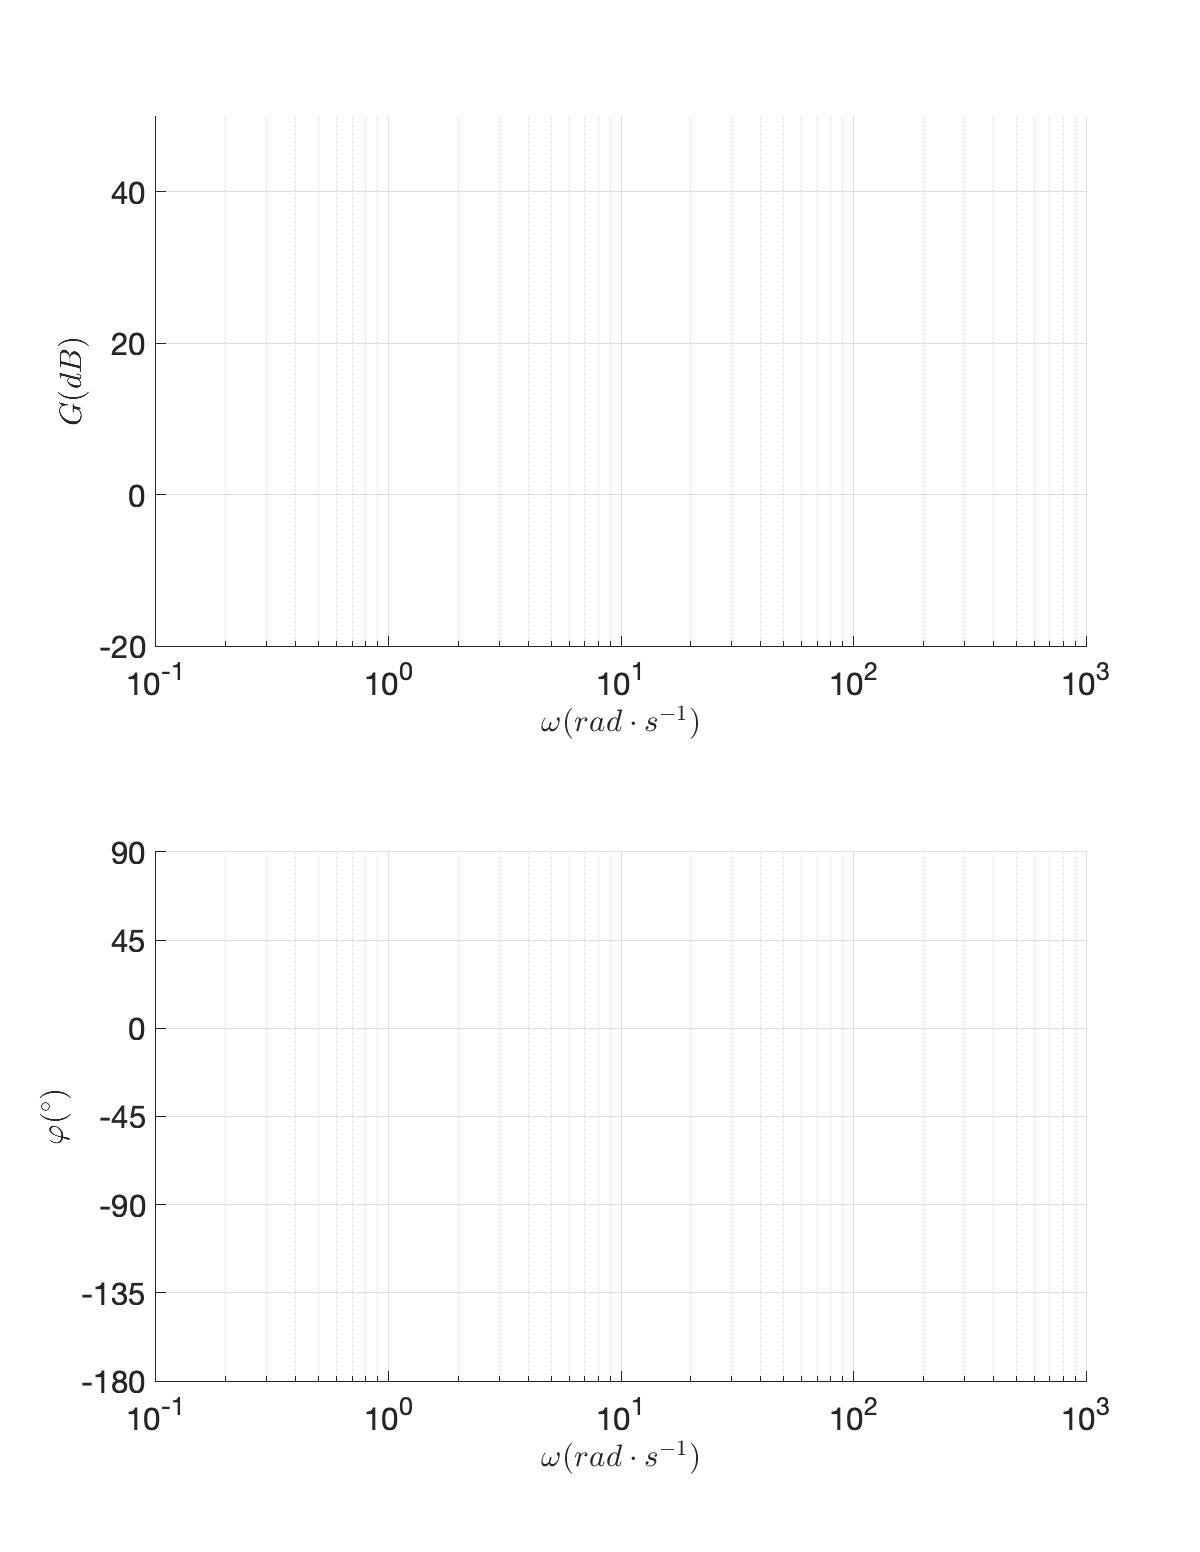
\includegraphics[width=0.9\textwidth]{images/bode_total_BO_0}
\end{center}
}


\question{En considérant toujours un retour unitaire, donner l'expression de $\varepsilon(p)=V_c(p)-V(p)$ en fonction de $V_c(p)$ et des constantes de la $FTBO$.}



\begin{texteCache}
\begin{align*}
\varepsilon(p)=V_c(p)-V(p)=\dfrac{V_c(p)}{1+FTBO(p)}=\dfrac{V_c(p)}{1+\dfrac{K_pK_mK_c}{\tau_i p}}
\end{align*}

\vspace{3cm}
\end{texteCache}

\question{Déterminer alors la précision du système dans ces deux cas.}


\begin{texteCache}

\begin{itemize}
\item Erreur statique : la transformée de Laplace d'un échelon d'amplitude $v_{c1}$ est $\dfrac{v_{c1}}{p}$. Alors,

\begin{align*}
\varepsilon_{sp1}=\lim_{p\rightarrow 0} p \varepsilon(p)=\lim_{p\rightarrow 0} p\dfrac{p\cdot v_{c1}}{p\left(1+\dfrac{K_pK_mK_c}{\tau_i p}\right)}=0
\end{align*}

\item Erreur de trainage : la transformée de Laplace d'un échelon d'amplitude $v_{c2}$ est $\dfrac{v_{c2}}{p}$. Alors,

\begin{align*}
\varepsilon_{sp2}=\lim_{p\rightarrow 0} p \varepsilon(p)=\lim_{p\rightarrow 0} \dfrac{p\cdot v_{c1}}{p^2\left(1+\dfrac{K_pK_mK_c}{\tau_i p}\right)}\\
=\lim_{p\rightarrow 0} \dfrac{v_{c1}}{p+\dfrac{K_pK_mK_c}{\tau_i}}\\
=\dfrac{v_{c1}\tau_i}{K_pK_mK_c}
\end{align*}
\end{itemize}
\end{texteCache}


\question{Entourer sur la courbe la zone qui montre que la
perturbation a été prise en compte. Préciser quelle non-linéarité (à
choisir parmi saturation, seuil, hystérésis) a été retenue. Conclure sur
la pertinence de l'asservissement de vitesse mis en place vis-à-vis des
performances attendues.}

\begin{minipage}{0.4\textwidth}
\ifthenelse{\boolean{corrige}}{
\begin{center}
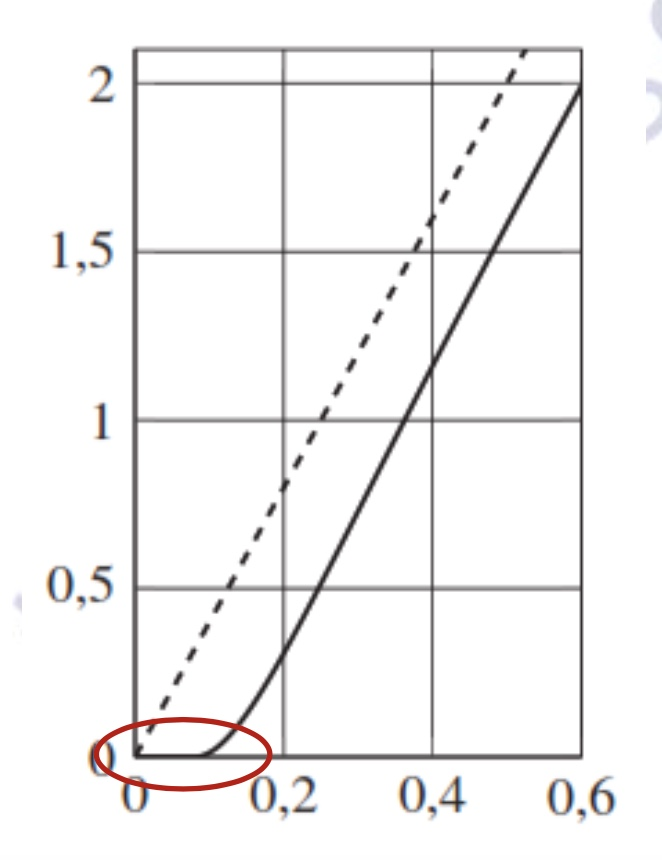
\includegraphics[width=0.9\textwidth]{images/NL1}
\end{center}
}
{
\begin{center}
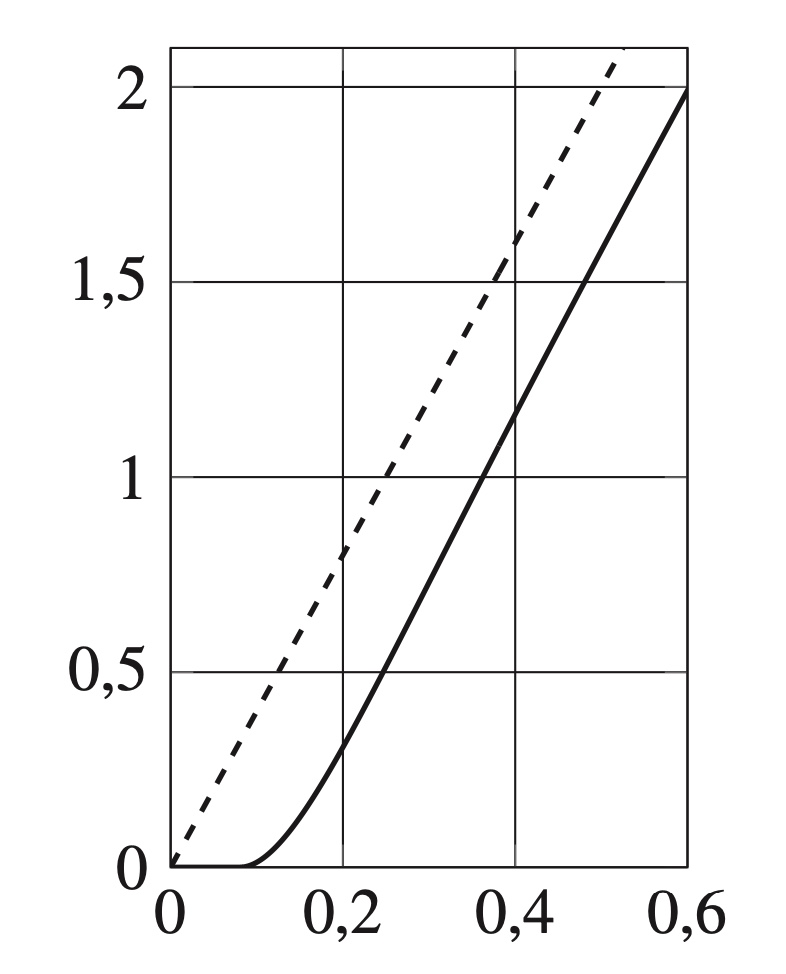
\includegraphics[width=0.9\textwidth]{images/NL0}
\end{center}
}
\end{minipage}
\begin{minipage}{0.6\textwidth}
\begin{texteCache}
La zone entourée montre que la perturbation a été prise en compte.

De type frottement sec, elle a été modélisée par un seuil
\end{texteCache}

\end{minipage}



\question{Donner le(s) exigence(s) sur le diagramme de la figure \ref{fig4} qui permettent de vérifier les performances dans ce cas. Donner alors les grandeurs quantifiable.}

\begin{texteCache}
Il s'agit de l'exigence de "pente sol" id 1.2.2. Le système doit pouvoir gravir une pente de 10 degrés.
\end{texteCache}


\question{Tracer l'évolution de \emph{C\textsubscript{m}}(\emph{t})
au cours du temps compte tenu de l'évolution souhaitée de
\emph{v}(\emph{t}). Préciser les valeurs caractéristiques sous forme
littérale, puis numérique.}



\begin{texteCache}
\begin{itemize}
\item \textbf{Pour $0 < t < \delta t$} 
\begin{align*}
\frac{dv(t)}{\text{dt}} = \frac{V_{\max}}{\delta t}
\end{align*} 
 
  donc~:

\begin{align*}
C_{m} = r_{\text{eq}}\left( M_{\text{eq}}\frac{V_{\max}}{\delta t} + F_{r,eq} \right) = 0,66\ Nm
\end{align*}

\item Pour \(\delta t < t < T-\delta t$ :
\begin{align*}
 v\left( t \right) = V_{\max}
\end{align*}

 donc~:

  \(C_{m} = C_{0} = r_{\text{eq}}\cdot F_{r,eq} =0,4 Nm\)

\item Pour $T-\delta t< t < T$ :

\begin{align*}
\frac{\text{dv}\left( t \right)}{\text{dt}} = - \frac{V_{\max}}{\delta t}
\end{align*}
  donc~:

  \(C_{m} = r_{\text{eq}}\left( - M_{\text{eq}}\frac{V_{\max}}{\delta t} + F_{r,eq} \right) = 0,136\ Nm\)
\end{itemize}

\end{texteCache}

\ifthenelse{\boolean{corrige}}{
\begin{center}
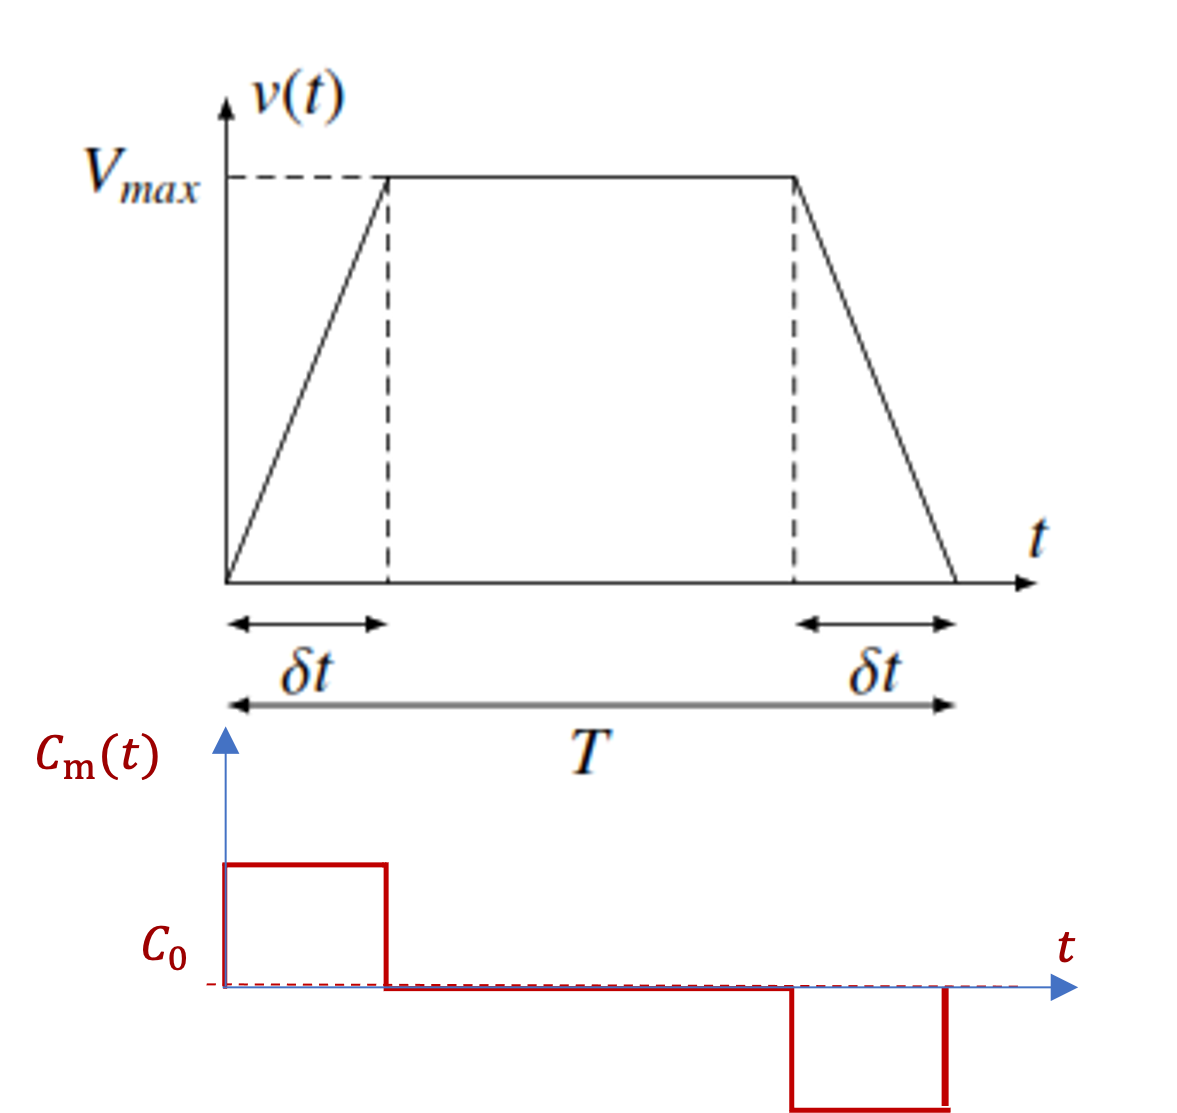
\includegraphics[width=0.9\textwidth]{images/couple_t_corrige}
\end{center}
}
{
\begin{center}
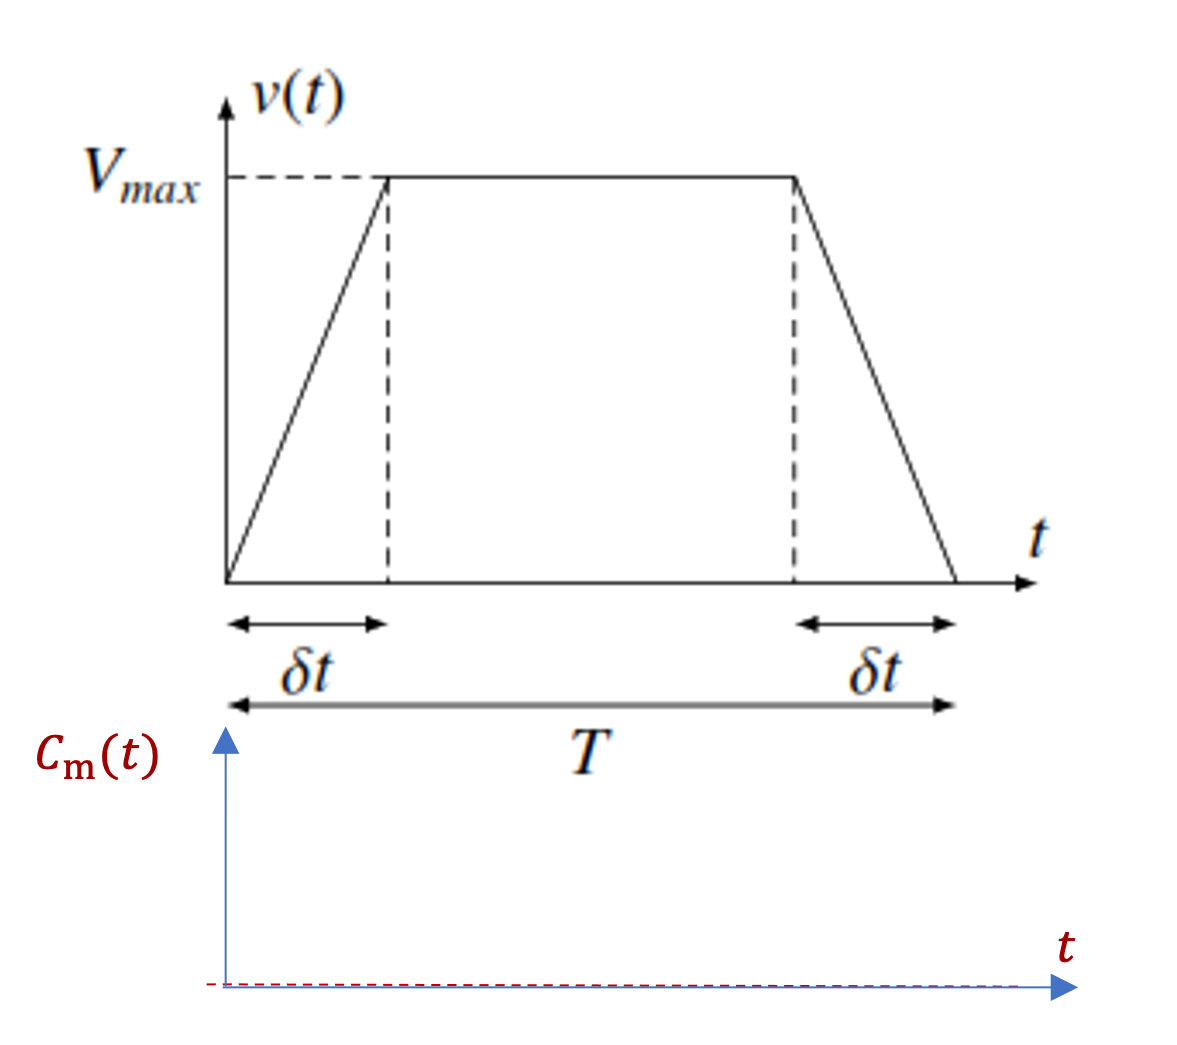
\includegraphics[width=0.9\textwidth]{images/couple_t_0}
\end{center}
}
\vspace{3cm}


\question{À l'aide des équations du moteur, déterminer le couple
maximal développé par un moteur lorsqu'il est alimenté sous 100 V.
Vérifier alors que la motorisation est adaptée à une montée en pente du
robot.}



\begin{texteCache}

  On reprend les équations (1) et (3)~:
  \(u_{m}\left( t \right) = R_{m}.i_{m}\left( t \right) + k_{m}.\omega_{m}\left( t \right)\)
  et \(C_{m}\left( t \right) = k_{m}.i_{m}\left( t \right)\)

  Soit
  \(C_{m}\left( t \right) = \frac{k_{m}}{R_{m}}u_{m}\left( t \right) - \frac{k_{m}^2}{R_{m}}\omega_{m}\left( t \right)\)

  Le couple moteur est maximal au démarrage, il vaut
  \(C_{\max} = \frac{k_{m}}{R_{m}}u_{m}\)

  Sous 100V, on trouve \(C_{\max} = 20\ Nm\) ce qui est très largement
  supérieur au couple nécessaire de 0,66 Nm trouvé à la question précédente.
  
  \vspace{3cm}

\end{texteCache}

